% !TeX root = lfgw.tex
\chapter{Literatur und Zitate automatisch verwalten}
\dictum[U. Eco, Name der Rose]{...}
\label{biblatex}
\autor{Lukas C. Bossert, Axel Kielhorn}

\noindent Sauberes zitieren in wissenschaftlichen Arbeiten ist wichtig,
nicht nur wenn man einen Ministerposten behalten möchte.
Ein Zitat sollte als solches gekennzeichnet werden und die Quelle muss genannt werden.

Das kann \LaTeX{} bereits mit Bordmitteln, 
allerdings ist es aufwändig,
die Literaturangaben entsprechend den Vorgaben zu formatieren.
Außerdem erfordert jeder Verlag und jedes Institut eine andere Formatierung.
Daher entstand bereits 1985 das Program \BibTeX,
das aus einer Datenbank und einer Formatierungsbeschreibung das Literaturverzeichnis erstellte.
Leider ist die Sprache zum Erstellen der Beschreibung nicht einfach zu verstehen
und Anpassung an die Formatierungswünsche ist schwierig.

Das Paket \biblatex{} wurde 2006 %JAHR  einfügen
von Philipp Lehmann entworfen und seitdem stetig weiterentwickelt. 
Von Haus aus bringt es bereits eine große Anzahl an Einstellmöglicheiten mit, 
die es erlauben auf die Vorgaben in den einzelnen Disziplinen einzugehen. 
Für weitere spezielle Eigenheiten in der Zitation und Bibliographie haben unzählige Mitglieder der \TeX -Community Stile und Erweiterungen entwickelt,
die dem  Paket als Option übergeben werden.\footcite{voss:bibliografien}

Bereits 2008 erschienen zwei Artikel in der DTK (Die TeXnische Komödie)\footcite{wassenhoven:dtk2008/2,wassenhoven:dtk2008/4}, 
die die Verwendung und Anpassung von \biblatex{} an die eigenen Wünsch beschreiben.
Beide Artikel können auf der Seite von \url{http://www.dante.de} heruntergeladen werden.

Das folgende Kapitel zeigt die Arbeit mit \biblatex: 
Zunächst wird erläutert, wie man eine Bibliografie-Datenbank erstellt und verwaltet (\cref{sec:bibliografiedatenbank}),
anschließend wie man die notwendigen Felder bestimmter Eintragstypen (Buch, Zeitschrift, Lexikon etc.) belegt, 
wie man im eigenen Text die Verweise einbaut (\cref{sec:zitate}) und
zum Schluss wie man eine oder mehrere (Teil"~)""Bibliografien erstellt.

Außerdem werden verschiedene Bibliografie-Stile vorgestellt,
die besonders für Geisteswissenschaftler relevant sind und die auf unterschiedliche Anforderungen in den verschiedenen Fachrichtungen Lösungen bereithalten (\cref{sec:bibliografie}).

Die offizielle Paket-Dokumentation von \biblatex{} gibt es nur in Englisch und sie umfasst mehr als 250~Seiten
Eine deutsche Übersetzung des Handbuchs ist Bestandteil von TeX-Live und im Verzeichnis 
\url{texmf-dist/doc/latex/translation-biblatex-de} zu finden.
Sie kann mit dem Befehl

\begin{lfgwcode}{label={lis:texdoc-biblatex}}
texdoc translation-bibtex
\end{lfgwcode}

in der Eingabeaufforderung bzw. dem Terminal aufgerufen werden.

Die Übersetzung entspricht nicht dem aktuellen Stand, ist aber in den meisten Fällen ausreichend.
Die Änderungen kann man im englischen Original im Anhang \enquote{Revision History} verfolgen.

Zusätzlich gibt es noch eine ausführliche Kurzeinführung\footcite{biblatex-tutorial} auf Englisch 
und eine sehr kurze deutsche Einführung\footcite{biblatex-bottcher}.

Die Einbindung von \biblatex{} in ein eigenes Dokument ist ganz einfach.

\begin{lfgwcode}{label={lis:biblatexkurz}}
\documentclass[headsepline,headinclude,10pt]{scrartcl}

\usepackage[german]{babel}
\usepackage[babel]{csquotes}
%
% Alphabetisch
%
%\usepackage[backend=biber,sortlocale=de,style=alphabetic]{biblatex}
%
% Numerisch
%
%\usepackage[backend=biber,sortlocale=de,style=numeric-comp]{biblatex}
%
% Author Year
%
\usepackage[backend=biber,sortlocale=de,style=authoryear]{biblatex}
%
% Literaturdatenbanken (mehrere sind möglich)
%
\bibliography{lfgw-bibliographie}

\begin{document}
  \printbibliography
\end{document}
\end{lfgwcode}

Beim Aufruf werden dem Paket die notwendigen Optionen übergeben

\begin{labeling}{sortlocale}
\item[backend]      Die Daten werden mit \biber{} verarbeitet, 
		ältere Versionen konnten auch mit dem backend \BibTeX{} arbeiten, das versteht jedoch kein Unicode.
\item[sortlocale]   Es wird nach deutschen Regeln sortiert (ß = ss).
		Zusätzlich gibt es noch die Option \verb+de_DE_phonebook+, dann werden die Umlaute (ä, ö, ü) wie (ae, oe, ue) sortiert.
\item[style]        Die Art der Formatierung (nur eine Auswahl der Wichtigsten):
    \begin{labeling}{authoryear}
    \item [alpahbetic] Erzeugt einen Verweis in der Form [Aut99] für das im Jahr 99 erschienen Werk des Authors.
    \item [numeric]    Erzeugt einen numerischen Verweis [12], diese Form ist in den Naturwissenschaften üblich.
    \item [authoryear] Der Verweis besteht aus dem vollen Namen des Authors und der Jahreszahl des Erscheinungsdatums.
    				Dieser Stil wir in diesem Dokument verwendet. Autor1999
    \item [-comp]      Einige Stile bieten eine \enquote{compressed} Version an, in der mehrere Verweise zusammengefasst werden. [1, 2-4]
    \end{labeling}
\end{labeling}

Mit dem Befehl \cs{bibliography} wählt man die Datenbank aus, es können auch mehrere sein.
An der gewünschten Stelle gibt der Befehl \cs{printbibliography} die formatierten Einträge aus.
Damit das funktioniert, 
muss nach dem ersten \TeX-Lauf des Program \biber{} mit dem Dokumentnamen (ohne Endung \texttt{.tex})
aufgerufen werden.

\begin{lfgwcode}{label={lis:texdoc-biber}}
biber Dokumentname
\end{lfgwcode}

Benutzt man zusätzlich noch das Paket \paket{hyperref}, 
kann man im PDF durch einen Klick auf den Literaturverweis direkt an die entsprechende Stelle im Literaturverzeichnis springen.
 
\section{Aufbau der Bibliografie-Datenbank}\label{sec:bibliografiedatenbank}
Eine Bibliografie-Datenbank ist zunächst nichts anderes als eine \meta{.text}-Datei,
die allerdings die Endung \meta{.bib} hat und ebenso mit jedem Texteditor bearbeitet werden kann.

\subsection{Grundlegender Aufbau}
Am Beispiel von \cite{voss:einfuehrung} sei der Aufbau eines Eintrags in der Bibliographiedatei erklärt (\cref{{lis:voss:einfuehrung}}):

\begin{lfgwcode}{label={lis:voss:einfuehrung}}
@Book{voss:einfuehrung,
 author    = {Herbert Voß}, 
 title     = {Einführung in \LaTeX},
 publisher = {DANTE~e.V. and Lehmanns Media},
 location  = {Berlin and Heidelberg},
 year      = {2016},
 edition   = {2},
}
\end{lfgwcode}

\begin{description}
 \item[1] \meta{@Book}: Damit wird das Wesen des Werks, der Publikationstypus, definiert, in diesem Fall handelt es sich um ein Buch; vgl. \cref{lit:publikationstypus}.
 \item[1] \meta{voss:einfuehrung}: Dies ist der \meta{Schlüssel}, den jeder Eintrag haben muss, um im Textdokument zitiert werden zu können.
 Dieser Schlüssel muss über alle Datenbanken eindeutig sein.
 \item[2-7] Alle Informationen zu einem Eintrag müssen in bestimmten Feldern geschrieben werden; z.\,B. \meta{author = {Herbert Voß}}: 
 Der Name des Autors des Buches wird in das Feld \marg{author} geschrieben. 
\end{description}
Jeder Eintrag beginnt mit dem Publikationstypus, alle weiteren Informationen sind innerhalb eines Klammerpaares.
\subsection{Schlüsselvergabe}
Anhand des \meta{Schlüssels} wird im Textdokument über einen \cs{cite}-Befehl (\cref{lit:cite-befehle}) das Werk eingebunden.
Ein solcher \meta{Schlüssel} muss innerhalb einer Bibliografie-Datei einmalig und eindeutig sein, 
da es ansonsten zu einer Fehlermeldung kommt.
In der Regel bieten Bibliografieverwaltungsprogramme wie JabRef eine Funktion an, anhand der man den \meta{Schlüssel} erzeugen kann. 

Es bietet sich an, den Namen des Autors und ein Kurztitel oder Nachname des (ersten) Autors und das Jahr der Publikation. 
Je kürzer und prägnanter ein \meta{Schlüssel} ist, desto weniger Tipparbeit bedeutet dies im Textdokument, zumal man den \meta{Schlüssel} zwar jederzeit ändern kann, aber diese Änderungen ebenfalls im Textdokument ausführen muss. 
Normalerweise bleibt daher der \meta{Schlüssel} für das gesamte Dokument gleich.

\subsection{Publikationstypen und ihre Datenfelder}\label{lit:publikationstypus}

\enquote{Die ganze Welt ist ein Buch} könnte man meinen, wenn man die unterschiedlichen Publikationstypen sieht.
Das stimmt aber nicht, die Welt besteht aus vielen Büchern (und einigen Artikeln).
Grundsätzlich ist alles, was nicht im einer Zeitschrift erschienen ist ein Buch.
Dabei is es egal, ob es sich um einen Kodex, eine Rolle oder einen Onlineartikel handelt,
wichtig sind nur der Titel und der Autor bzw. Editor.

Zu jedem Publikationstypus gibt es notwendige und optionale Felder.
Die Art des Dokuments hängt dann von den vorhandenen Informationen ab, 
man wählt den Typus, für den alle notwendigen Informationen bekannt sind.
Grundsätzlich ist es eine gute Idee alle bekannten Informationen an einer Stelle (der Literaturdatenbank) zu sammeln,
auch wenn der verwendete Stil diese Information nicht nutzt.
Dazu gehört auch die Information aus welcher Bibliothek das Werk entliehen wurde, 
falls man später noch einmal darauf zugreifen muss.

Zusätzliche Bibliografiestile können weitere Publikationstypen bereithalten,
wie z.\,B. der Stil \meta{arthistory-bonn} für einen ›Ausstellungskatalog‹ den Eintrag \meta{@exhibcatalog} 
und \meta{@movie} für einen Film im Stil \meta{fiwi}.

Die meisten Publikationstypen benötigen folgende Felder:
\meta{author} oder \meta{editor}
\meta{title},
\meta{year} oder \meta{date}.

\subsubsection{Bücher (Monografie, Sammmelband)}

Zu den buchartigen Werken gehören: 

\begin{labeling}{\meta{@mvproceedings}}
\item[\meta{@book}]         Ein einzelnes Buch mit einem oder mehreren Autoren die für das Gesamtwerk verantwortlich sind.
\item[\meta{@mvbook}]       Ein mehrbändiges Buch.
%
\item[\meta{@collection}]   Ein Buch mit mehreren Autoren, die für einzelne Abschnitte verantwortlich sind.
        Die einzelnen Abschnitte werden über \meta{@incollection} identifiziert. Das Geamtwerk hat einen \meta{editor}.
\item[\meta{@mvcollection}] Eine mehrbändige \meta{@collection}.
%
\item[\meta{@reference}]    Eine Möglichkeit Lexika hervorzuheben, 
        wird jedoch in den Standardstilen wie eine \meta{@ollection} behandelt.
\item[\meta{@mvreference}]
%
\item[\meta{@proceedings}]  Ein Tagungsband. Anders als bei einer \meta{@ollection} ist hier kein \meta{editor} erforderlich.
        Optional kann eine \meta{organization} angegeben werden.
\item[\meta{@mvproceedings}] Ein mehrbändiger Tagungsband.
%
\item[\meta{@inbook}]       Ein Teil eines Buches.
\item[\meta{@incollection}] Ein Teil einer \meta{@collection}.
\item[\meta{@inreference}]
\item[\meta{@proceedings}]
%
\item[\meta{@booklet}]      Ein Buch, das nicht von einem Verlag verlegt wurde.
        Anstelle eines \meta{author}s kann auch ein \meta{editor} angegeben werden.
        Die Art der Veröffentlichung kann im Feld  \meta{howpublished} angegeben werden
\item[\meta{@manual}]       Ein Handbuch. Anders als beim \meta{@booklet} können \meta{author} und \meta{editor} entfallen.
\item[\meta{@misc}]         Bei diesem Typus können \meta{author}, \meta{editor} und \meta{year} entfallen.
\item[\meta{@patent}]       Die Patentnummer \meta{number} ist zusätzlich erforderlich.
\item[\meta{@online}]       Anstelle eines \meta{author}s kann auch ein \meta{editor} angegeben werden.
        Zusätzlich ist die Angabe einer \meta{url} erforderlich.
\item[\meta{@report}]       Zusätzlich ist die Angabe einer \meta{institution} und des \meta{type} erforderlich.
\item[\meta{@thesis}]       Eine Dissertation, die erforderlichen Daten entsprechen dem \meta{report}.
\item[\meta{@unpublished}]  Ein noch nicht veröffentlichtes Buch.
\end{labeling}

\subsubsection{Zeitschriften (Artikel, Rezensionen)}

\begin{labeling}{\meta{@mvproceedings}}
\item[\meta{@article}]    Ein Artikel, der in einer Zeitschrift erschienen ist.
        Die Zeitschrift wird im Feld \meta{journaltitle} angegeben.
\item[\meta{@review}]     Eine Rezension (von Büchern, Filmen etc.)
        Kann von bestimmten Stilen besonders formatiert werden, 
        ist in den Standardstilen identisch mit \meta{article}
\item[\meta{@periodical}] Die komplette Zeitschrift, der \meta{editor} ist optional.
\end{labeling}

\subsubsection{Gesetze und Normen}

Für die folgenden Typen gibt es in den Standardstilen keine besondere Formatierung,
sie werden als \meta{misc} behandelt.
Spezielle fachbezogenen Bibliografiestile können eine angepasste Formatierung benutzen.

\begin{labeling}{\meta{@mvproceedings}}
\item[\meta{@legislation}]      Gesetzestexte
\item[\meta{@commentary}]       Kommentare zu Gesetzestexten
\item[\meta{@standard}]         Normen
\end{labeling}

\subsubsection{Übersicht: Datenfelder}
Theoretisch und technisch können (fast) alle Datenfelder für alle Publikationstypen genutzt werden.
Allerdings ist dies nicht immer sinnvoll, wie z.\,B. eine Seitenangabe bei einer Webseite keinen logischen Mehrwert hat.

Neben den hier aufgeführten Feldern gibt es noch weitere, die ein Dokument
genauer beschreiben können.

\begin{labeling}{\meta{organization}}
\item[Namen]    \biblatex{} betreibt einen großen Aufwand um Namen richtig zu formatieren.
        Ein Name besteht aus dem Vornamen \meta{first} und dem Nachname \meta{last}.
        Zusätzlich kann er noch einen Namenszusatz \meta{von} und einen Namensanhang \meta{Jr} erhalten.
        Namen werden für \meta{author} und \meta{editor} verwendet.
        Mehrere Namen werden durch ein \meta{and} verbunden.
\item[Datum] Ein Datum kann gemäß ISO 8601 angegeben werden (yyyy-mm-dd). 
\end{labeling}

\begin{labeling}{\meta{organization}}
\item[\meta{title}]       Der Titel des Werks, in den meisten Fällen erforderlich.
\item[\meta{author}]      Der Autor des Werks, in den meisten Fällen erforderlich.
\item[\meta{editor}]      Der Herausgeber, wird in einigen Typen anstelle des \meta{author}s benutzt.
\item[\meta{translator}]  Der Übersetzer.
\item[\meta{publisher}]   Der Verlag.
\item[\meta{organization}] Alternativ zu \meta{publisher} z.\,B. eine Organisation oder eine Firma.
\item[\meta{institution}] Alternativ zu \meta{publisher} z.\,B. eine Schule oder Universität.
\item[\meta{type}]        Art des \meta{@report}s oder der \meta{@thesis}.
%
\item[\meta{chapter}]     Das zitierte Kapitel.
\item[\meta{pages}]       Eine Seitenzahl oder ein Bereich.
%
\item[\meta{year}]        Erscheinungsjahr (bei Büchern).
\item[\meta{month}]       Erscheinungsmonat (bei Zeitschriften).
\item[\meta{issue}]       Die Ausgabe eines Buches oder einer Zeitschrift.
        Kann eine Zahl oder eine Text sein.
\item[\meta{number}]      Die Nummer eines Buches oder einer Zeitschrift in einer Serie.
        Kann eine Zahl oder eine Text sein.
%
\item[\meta{isbn}]  International Standard Book Number. 
\item[\meta{issn}]  International Standard Serial Number. 
\end{labeling}

\subsection{Literaturdatenbank mit JabRef}

Natürlich \emph{kann} man eine Literaturdatenbank mit einem normalen Texteditor erstellen.
Sehr viel bequemer ist es aber, ein darauf spezialisiertes Programm zu benutzen.
Das Programm wurde 2003 in Java (daher \enquote{Ja}) geschrieben um bibliothekarische Referenzen zu verwalten
(daher das \enquote{bRef}).

Zuerst wird eine neue Datenbank angelegt (Bild~\ref{fig:lis:jabref1}).

\begin{figure}
  
\includegraphics{Jabref1}
  \caption{Eine neue Literaturdatenbank mit JabRef}
  \label{fig:lis:jabref1}
\end{figure}

Durch einen Klick auf das Feld mit dem $+$-Zeichen wird ein neuer Eintrag angelegt.
Hier kann der Typus aus einer Liste ausgewählt werden. (Bild~\ref{fig:lis:jabref2})
JabRef kennt die notwendigen Einträge und gibt einen Fehler aus, wenn einer fehlt.

\begin{figure}
  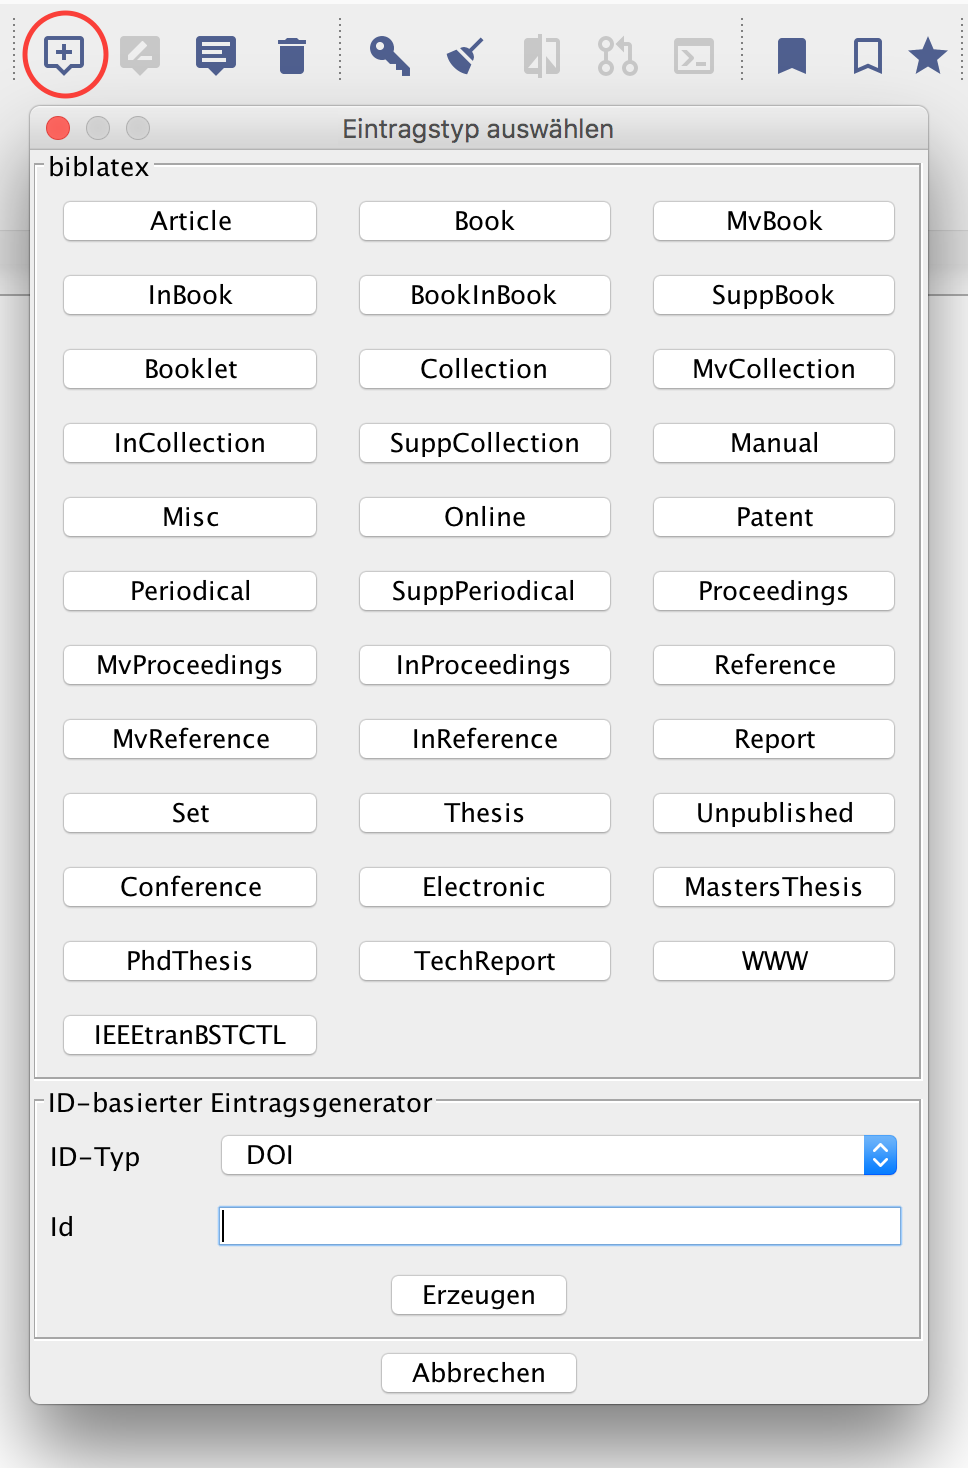
\includegraphics[width=\textwidth]{Jabref2}
  \caption{Auswahl des Dokumenttypus}
  \label{fig:lis:jabref2}
\end{figure}

Als besondere Funktion kann JabRef nach Eingabe der \meta{ISBN} oder des \meta{DOI} die Daten
aus dem Internet abfragen. Dazu dient der schwarze Kasten mit dem Pfeil nach unten. (Bild~\ref{fig:lis:jabref3})
Meistens müssen die Daten noch nachbearbeitet werden, aber es spart viel Tipparbeit.

\begin{figure}
  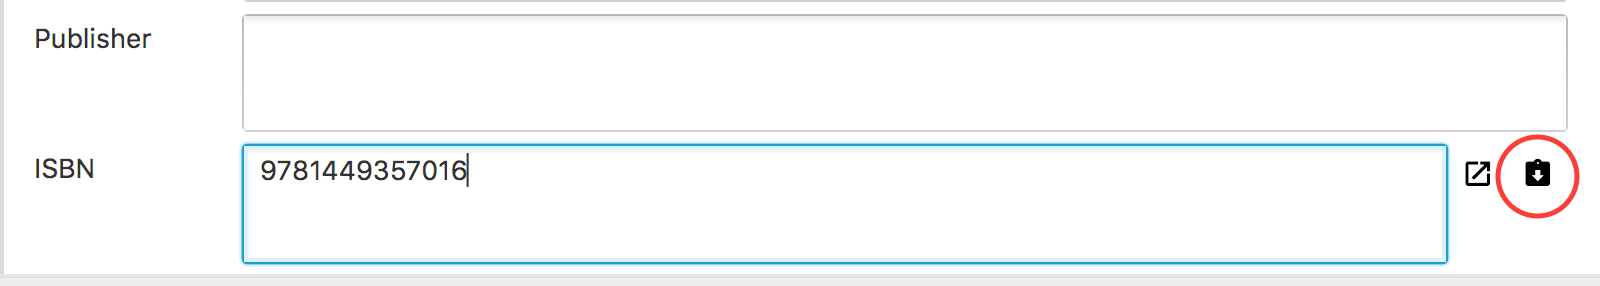
\includegraphics[width=\textwidth]{Jabref3}
  \caption{Abfrage der Daten aus dem Internet.}
  \label{fig:lis:jabref3}
\end{figure}

\section{Zitate}\label{sec:zitate}\label{lit:cite-befehle}

Normale Zitate werden mit dem Befehl \cs{cite} ausgeführt:
\begin{lfgwcode}{label={lis:XXX}}
\cite*@\oarg{Präfix}\oarg{Suffix}\marg{Schlüssel}@*
\end{lfgwcode}

Während \meta{Präfix}  eine kurze Anmerkung \emph{vor} die Zitation (z.\,B. \enquote{Vgl.}) setzt, 
wird  \meta{Suffix} für gewöhnlich für Seitenzahlen verwendet.
Ist nur ein optionales Argument definiert, 
dann wird es als \oarg{Suffix} behandelt.
\begin{lfgwcode}{label={lis:code:cite}}
\cite*@\oarg{Suffix}\marg{Schlüssel}@*
\end{lfgwcode}
Der \meta{Schlüssel} korrespondiert mit dem Schlüssel der Bibliografie-Datei.

\begin{lfgwexample}{label={lis:example:cite}}
\enquote{Der öffentliche Raum ist Teil einer Stadt.}\cite{Osland2016}.
\end{lfgwexample}

\minisec{\cs{cites}}
Möchte man hingegen mehrere Autoren oder Werke zitieren, 
gibt es zwei Möglichkeiten:
Entweder kann man dies durch die Komma-getrennte Reihung der \marg{Schlüssel} machen,
was jedoch den Nachteil hat, dass man für die einzelnen \marg{Schlüssel} keine \oarg{Präfixe} oder \oarg{Suffixe} definieren kann.

Die andere Möglichkeit sieht vor, den Befehl \cs{cites} zu verwenden, 
bei dem für jeden Autor\,/\,jedes Werk sowohl \oarg{Präfixe} als \oarg{Suffixe} definiert werden kann.
Zudem lässt sich für die gesamte Reihung ein \oarg{Präfix} und ein \oarg{Suffix} festlegen:
\begin{lfgwcode}{label={lis:code:cites}}
\cite{Schlüssel1, Schlüssel2, Schlüssel3}
\cites(Prä-Präfix)(Suf-Suffix)
  *@\oarg{Präfix}\oarg{Suffix}\marg{Schlüssel1}@*%
  *@\oarg{Präfix}\oarg{Suffix}\marg{Schlüssel2}@*%
  *@\oarg{Präfix}\oarg{Suffix}\marg{Schlüssel3}\ldots@*
\end{lfgwcode}
\begin{lfgwexample}{label={lis:example:cites}}
Der öffentliche Raum ist Teil einer Stadt \cites(vgl.)(){Osland2016} {Evangelidis2014}.
\end{lfgwexample}
% Leerzeichen vor Evangelidis2014 erforderlich, sonst kein Umbruch (Axel).
 
 
\minisec{\cs{parencite}}
Manchmal soll die Zitation in Klammern stehen.
Um dies nicht händisch in runde Klammern setzen zu müssen (und ggf. die \enquote{Klammerschachtelregel} zu verletzen),
kann dafür der Befehl  \cs{parencite} verwendet werden:
\begin{lfgwcode}{label={lis:code:parencite}}
\parencite*@\oarg{Suffix}\marg{Schlüssel}@*
\end{lfgwcode} 
Mit diesem Zitationsbefehl wird die korrekte Ordnung von korrespondierenden Klammern berücksichtigt.
\begin{lfgwexample}{label={lis:example:parencite}}
\enquote{Der öffentliche Raum ist Teil einer Stadt.} \parencite{Osland2016}
\end{lfgwexample}

\minisec{\cs{parencites}}
Ebenso lassen sich auch mehrere Zitationen mit Klammern umschließen.
Dies wird mittels \cs{parencites} umgesetzt:
\begin{lfgwcode}{label={lis:code:parencites}}
\parencites(Prä-Präfix)(Suf-Suffix)%
*@\oarg{Präfix}\oarg{Suffix}\marg{Schlüssel}@*%
*@\oarg{Präfix}\oarg{Suffix}\marg{Schlüssel}@*%
*@\oarg{Präfix}\oarg{Suffix}\marg{Schlüssel}\ldots@*
\end{lfgwcode}
\begin{lfgwexample}{label={lis:example:parencites}}
Der öffentliche Raum ist Teil einer Stadt.\parencites(s.)(){Osland2016}
[vgl.][]{Evangelidis2014}.
\end{lfgwexample}
% "%" vor Evangelidis2014 nicht erforderlich, irritiert im Beispiel (Axel).

\minisec{\cs{textcite}}
Neben den bereits angeführten \cs{cite}-Befehlen gibt es eine dritte Möglichkeit der Zitationsangabe:
\cs{textcite} ist vor allem für die Fälle zu nutzen, 
bei denen der Autor\,/\,das Werk im Fließtext genannt sein soll, 
aber die weiteren Angaben (Publikationsjahr, Seitenangabe) nur in runden Klammern dahinter.
\begin{lfgwcode}{label={lis:code:textcite}}
\textcite*@\oarg{Suffix}\marg{Schlüssel}@*
\end{lfgwcode} 

\begin{lfgwexample}{label={lis:example:textcite}}
Der öffentliche Raum ist Teil einer Stadt, sagt \textcite{Osland2016}.
\end{lfgwexample}

\minisec{\cs{textcites}}
Wiederum können mehrere Autoren\,/\,Werke mittels \cs{textcites} gelistet werden:
\begin{lfgwcode}{label={lis:code:textcites}}
\textcites(Prä-Präfix)(Suf-Suffix)%
  *@\oarg{Präfix}\oarg{Suffix}\marg{Schlüssel}@*%
  *@\oarg{Präfix}\oarg{Suffix}\marg{Schlüssel}@*%
  *@\oarg{Präfix}\oarg{Suffix}\marg{Schlüssel}\ldots@*
\end{lfgwcode}
\begin{lfgwexample}{label={lis:example:textcites}}
Der öffentliche Raum ist Teil einer Stadt, sagen \textcites{Osland2016}
[vgl.][]{Evangelidis2014}.
\end{lfgwexample}
% "%" vor Evangelidis2014 nicht erforderlich, irritiert im Beispiel (Axel).

\minisec{\cs{footcite}}
Darüberhinaus gibt es weitere \cs{cite}-Befehle, 
die die Einbettung der Zitation beeinflussen. 
Zunächst kann man mit \cs{footcite} die Zitation direkt als eigene Fußnote setzen:
 \begin{lfgwcode}{label={lis:code:footcite}}
\footcite*@\oarg{Präfix}\oarg{Suffix}\marg{Schlüssel}@*
\end{lfgwcode}
\begin{lfgwexample}{label={lis:example:footcite}}
\enquote{Der öffentliche Raum ist Teil einer Stadt.}\footcite{Osland2016}
\end{lfgwexample}
\cs{footcite} ist das Äquivalent zu \lstinline/\footnote{\cite{Osland2016}.}/
was jedoch manche (überflüssige) Tipparbeit spart.

\minisec{\cs{footcites} }
Für mehrere Autoren\,/\,Werke in einer Fußnote gibt es auch \cs{footcites}:
\begin{lfgwexample}{label={lis:example:footcites}}
\enquote{Der öffentliche Raum ist Teil einer Stadt.}\footcites(s.)(){Osland2016}
[vgl.][]{Evangelidis2014}
\end{lfgwexample}
% "%" vor Evangelidis2014 nicht erforderlich, irritiert im Beispiel (Axel).
 
\minisec{\cs{smartcite}}
Eine clevere Art und Weise Zitationen als Fußnote zu setzen,
bietet der Befehl \cs{smartcite}.
 \cs{smartcite} reagiert auf die Umgebung des Befehls:
 Befindet sich \cs{smartcite} innerhalb des Fließtexts wird es wie \cs{footcite} behandelt 
 und die Zitation in eine Fußnote setzen. 
Wird die Zitation allerdings in einer Fußnote aufgerufen,
erfolgt die Ausgabe nach dem Schema von \cs{cite}. 
\begin{lfgwcode}{label={lis:code:smartcite}}
\smartcite*@\oarg{Suffix}\marg{Schlüssel}%@*
\end{lfgwcode} 

\begin{lfgwexample}{label={lis:example:smartcite}}
Der öffentliche Raum ist Teil einer Stadt.\smartcite{Osland2016} 
Eventuell aber zugangsbeschränkt. \footnote{\smartcite[vgl.][] {Evangelidis2014}.}
\end{lfgwexample}
%%% Smartcite in der Fußnote funktioniert hier nicht. 

\minisec{\cs{smartcites}}
Wiederum gibt es analog auch den Befehl \cs{textcites}, 
um mehrere Autoren\,/\,Werke clever zu zitieren:
\begin{lfgwcode}{label={lis:code:smartcites}}
\smartcites(Prä-Präfix)(Suf-Suffix)%
  *@\oarg{Präfix}\oarg{Suffix}\marg{Schlüssel}@*%
  *@\oarg{Präfix}\oarg{Suffix}\marg{Schlüssel}@*%
  *@\oarg{Präfix}\oarg{Suffix}\marg{Schlüssel}\ldots@*
\end{lfgwcode}
\begin{lfgwexample}{label={lis:example:smartcites}}
Der öffentliche Raum ist Teil einer Stadt.\smartcites{Osland2016} {Evangelidis2014} 
Eventuell aber zugangsbeschränkt.\footnote{ \smartcites{Osland2016}
[cf.][]{Evangelidis2014}.}
\end{lfgwexample}

\minisec{\cs{autocite}}
Mit  \cs{autocite} ist eine individuelle und flexible Zitationsangabe möglich,
indem man in der Präambel steuert,
wie \cs{autocite} ausgegeben werden soll.
Für gewöhnlich stehen folgende Optionen zur Verfügung:
\begin{labeling}{footnote}
	\item[plain] Ausgabe wie \cs{cite}
	\item[inline]Ausgabe wie \cs{parencite}
	\item[footnote]Ausgabe wie \cs{footcite}
\end{labeling}
\begin{lfgwcode}{label={lis:code:autocite}}
\autocite*@\oarg{Präfix}\oarg{Suffix}\marg{Schlüssel}@*
\end{lfgwcode} 

\begin{lfgwexample}{label={lis:example:autocite}}
Der öffentliche Raum ist Teil einer Stadt \autocite{Osland2016} 
\end{lfgwexample}

\minisec{\cs{fullcite} \cs{footfullcite}}
Mit den Befehlen \cs{fullcite} und \cs{footfullcite} werden zwei Möglichkeiten gegeben,
mit denen man den kompletten Bibliographie-Eintrag in den Fließtext bzw. in die Fußnote schreiben kann.
\begin{lfgwcode}{label={lis:code:footfullcite}}
\fullcite*@\oarg{Präfix}\oarg{Suffix}\marg{Schlüssel}@*
\footfullcite*@\oarg{Präfix}\oarg{Suffix}\marg{Schlüssel}@*
\end{lfgwcode} 

\begin{lfgwexample}{label={lis:example:footfullcite}}
Der öffentliche Raum ist Teil einer Stadt.\footfullcite{Osland2016}
Das steht auch geschrieben bei \fullcite{Evangelidis2014}
\end{lfgwexample}



\minisec{\cs{citeauthor} \cs{citetitle}}
Neben den \enquote{geläufigen} \cs{cite}-Befehlen kann man auch nur den oder die Autoren zitieren 
und ebenso nur den Werktitel.
Dies funktioniert für den Fließtext und für Fußnoten gleichermaßen, zuerst der Author:
\begin{lfgwcode}{label={lis:code:citeauthor}}
\citeauthor *@ \oarg{Präfix}\oarg{Suffix}\marg{Schlüssel} @*
\end{lfgwcode} 
  und dann seine Werke:
\begin{lfgwcode}{label={lis:code:citetitle}}
\citetitle *@\oarg{Präfix}\oarg{Suffix}\marg{Schlüssel} @*
\end{lfgwcode} 

\begin{lfgwexample}{label={lis:example:citetitle}}
Der öffentliche Raum ist Teil einer Stadt sagt \citeauthor{Osland2016} in \citetitle{Osland2016}.
\footnote{Der öffentliche Raum ist Teil einer Stadt sagt \citeauthor{Osland2016} in \citetitle{Osland2016}.}
\end{lfgwexample}


\minisec{\cs{nocite}}
Möchte man einen Eintrag nicht als Zitation im Text haben, 
aber auf die Auflistung in der Bibliographie nicht verzichten,
dann kann man \cs{nocite}\marg{Schlüssel} verwenden.
Die Zitation wird damit \enquote{unsichtbar} zitiert:
Sie taucht nicht im Fließtext aber dennoch in der Bibliographie auf.

Mit dem Befehl \cs{nocite}\marg{*} werden alle Werke aus der
Literaturdatenbank in das Literaturverzeichnis übernommen.


\section{Bibliografie-Stile}\label{sec:bibliografiestile}
Mit der zunehmenden Anwendung von \LaTeX{} in den Geisteswissenschaften steigt auch die Frage nach den \enquote*{passenden} Zitierstilen für die unterschiedlichen Fachgebiete:
Sei es Archäologie, Alte Geschichte, Filmwissenschaft, Theologie usw.
\subsection{Standardstile von \biblatex}

Es wäre schön, wenn man sich auf Zitate gemäß DIN~1505, ISO~690 oder APA beschränken könnte.
Leider hat jede Zeitschrift und jedes Hochschulinstitut einen eigenen Zitierstil.
Die folgenden \biblatex-Stile sollten einen Großteil der Anforderungen abdecken, oder sich leicht anpassen lassen.

\begin{labeling}{historische-zeitschrift}
  \item[biblatex-apa6]      APA Style Guide (6th Edition)
  \item[biblatex-apa]       APA Style Guide (7th Edition)
  \item[biblatex-dw]        Bietet zwei Optionen: \lstinline/style=authortitle-dw/ und \lstinline/style=footnote-dw/.
  \item[biblatex-archaeology] Regeln des \enquote{Deutschen Archäologischen Instituts} (sehr viele Optionen)
  \item[geschichtsfrkl]     Regeln der Historiker der Universität Freiburg
  \item[historische-zeitschrift] Regeln der \enquote{Historischen
    Zeitschrift}
  \item[biblatex-historian] Angelehnt an das \enquote{Chicago Manual of Style}
  \item[biblatex-arthistory-bonn] Regeln des \enquote{Kunsthistorischen Instituts der Universität Bonn}.
  \item[biblatex-fiwi]      Der \biblatex-Zitierstil für Filmwissenschaftler bietet zwei Optionen: \lstinline/style=fiwi/ und \lstinline/style=fiwi2/.
\end{labeling}

\minisec{Weitere nützliche Bibliografiestile}

TeX-Live enthält ca. 50 angepasste Bibliografiestile für spezielle Anwendungen, 
nicht alle davon sind für deutschsprachige Nutzer relevant.


\begin{labeling}{historische-zeitschrift}
\item[biblatex-anonymous] Zitieren anonymer Werke.
\item[biblatex-bwl]       Regeln für den BWL-Studiengang an der FU Berlin.
\item[biblatex-chem]      Für Chemiker
\item[biblatex-chicago]   Nach den Regeln des \enquote{Chicago Manual of
  Style}
\item[biblatex-ext]       \biblatex{} Erweiterungen
\item[biblatex-iso690]    Regeln der ISO 690
\item[biblatex-jura2]     Speziell für Juristen
\item[biblatex-lni]       Regeln der \enquote{Lecture Notes in Informatics}
\item[biblatex-luh-ipw]   Regeln des Instituts für Politische Wissenschaft der Universität Hannover
\item[biblatex-manuscripts-philology]
\item[biblatex-mla]       Regeln der \enquote{Modern Language Association}
\item[biblatex-musuos]    Regeln des \enquote{Instituts für Musik und
  Musikwisenschaften der Universität Osnabrück}
\item[biblatex-nature]    Regeln der Zeitschrift \enquote{Nature}
\item[biblatex-oxref]     Regeln des \enquote{Oxford Guide to Style}
\item[biblatex-phys]      Regeln der AIP (American Institute of Physics) und der APS (American Physical Society)
\item[biblatex-sbl]       Regeln der \enquote{Society of Biblical Literature}
\item[biblatex-science]   Regeln der Zeitschrift \enquote{Science}
\item[biblatex-socialscienceshuberlin] Regeln der Sozialwissenschaften der Humboldt-Universität zu Berlin
\item[biblatex-trad]      Nachbildung der BibTeX Formatierung
\end{labeling}

\subsection{Spickzettel}

\biblatex{} ist inzwischen so leistungsfähig geworden, dass man sich nicht alles merken kann.
Das dachte sich auch Clea F. Rees und schuf im Jahre 2017 das \Package{biblatex-cheatsheet}.
Hier hat man alle \cs{cite} Befehle auf einen Blick und kann auch die verfügbaren Datenbank Felder schnell nachschlagen.

\subsection{Schlüsselbund}

Entscheidend für die Benutzung von \biblatex{} sind die Zitierschlüssel.
Gerade bei gewachsenen Datenbanken,
oder wenn wie in diesem Buch mehrere Autoren zusammenarbeiten,
wünscht man sich ein Literaturverzeichnis mit den dazugehörigen Schlüsseln.

Hier hilft das Paket \Package{showkeys} weiter.
In Verbindung mit einer kleinen \LaTeX-Datei erstellt es ein Literaturverzeichnis mit den dazugehörigen Schlüsseln.

\begin{lfgwcode}{label={lis:Zitierschluessel}}
\documentclass[headsepline,headinclude,10pt]{scrartcl}
\usepackage[a4paper, left=5cm]{geometry} % breiter Rand
\usepackage{showkeys}                    % Zitierschlüssel zeigen
\usepackage[german]{babel}
\usepackage[babel]{csquotes}
%
% Alphabetisch
%
%\usepackage[backend=biber,sortlocale=de,style=alphabetic]{biblatex}
%
% Numerisch
%
%\usepackage[backend=biber,sortlocale=de,style=numeric-comp]{biblatex}
%
% Author Year
%
\usepackage[backend=biber,sortlocale=de,style=authoryear]{biblatex}
%
% Literaturdatenbanken (mehrere sind möglich)
%
\bibliography{lfgw-bibliographie}

\begin{document}
\nocite{*} % Alle Quellen ausgeben
\printbibliography
\end{document}
\end{lfgwcode}

Wichtig ist hier die Zeile 2, damit der Zitierschlüssel nicht außerhalb des Blattes gedruckt wird.
Zeile 3 aktiviert dann die Ausgabe der Schlüssel im linken Rand.
Idealerweise wählt man die gleiche Sortierreihenfolge wie im fertigen Dokument.

Das Paket \Package{showkeys} kann man auch im normalen Dokument benutzen, 
es zeigt zusätzlich auch die definierten \cs{label} an.

\section{An die Arbeit}

Wenn man mit einer integrierten Entwicklungsumgebung arbeitet, 
muss man sich normalerweise keine weiteren Gedanken machen,
evtl. ist es erforderlich von \Package{bibtex} auf \Package{biblatex} umzuschalten.

In TeXWorks geschieht das über ein Menü links oben (Bild~\ref{fig:lis:TWbiber}).

\begin{figure}
  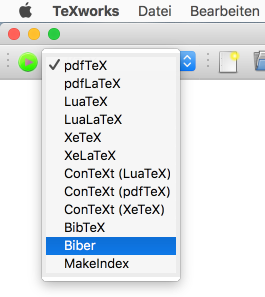
\includegraphics[width=0.7\textwidth]{TW-Biber}
  \caption{Biber in TeXWorks auswählen}
  \label{fig:lis:TWbiber}
\end{figure}

In TexStudio schaltet man im Menü Bibliographie auf \BibLaTeX{} um (Bild~\ref{fig:lis:TSbiblatex}).

\begin{figure}
  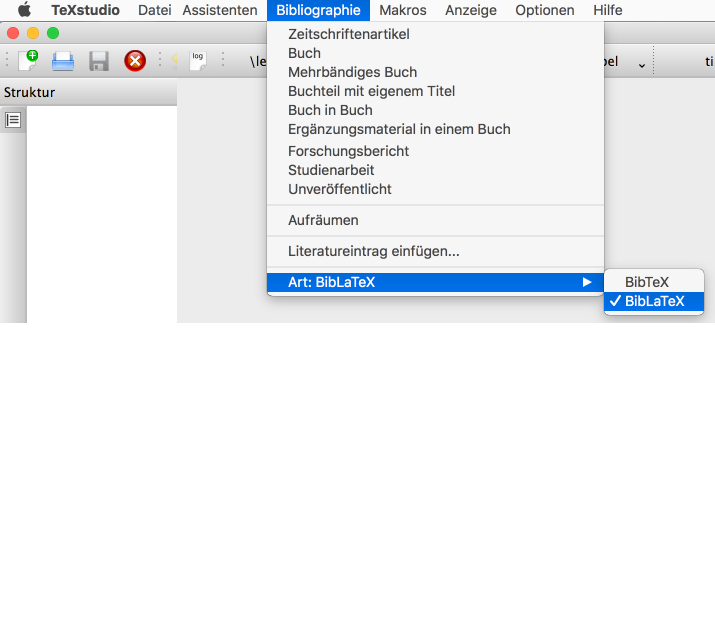
\includegraphics[width=\textwidth]{TS-Biblatex}
  \caption{Biber in TeXStudio auswählen}
  \label{fig:lis:TSbiblatex}
\end{figure}

Auf der Kommandozeile ist es auch nicht schwieriger:

\begin{lfgwcode}{label={lis:bibercmd}}
> pdflatex dokumentname
> biber dokumentname
> pdflatex dokumentname
\end{lfgwcode}

Zuerst wird das Dokument mit \Package{pdflatex} (oder \Package{lualatex}) übersetzt,
dann \biber{} aufgerufen und zum Schluss da Dokument noch einmal übersetzt.

Fehler können auftreten, wenn ein Schlüssel mehrfach verwendet wird, 
oder die öffnenden und schließenden Klammern nicht zusammenpassen.

\section{Ein Beispiel für Historiker: Quellen und Sekundärliteratur}\label{sec:bibliografie}
\index{Quellenverzeichnis}
\index{Bibliographie}
\index{Literaturverzeichnis}
\index{Sekundärliteratur}


%\begin{lfgwcode}{}  % läuft bei mir nicht - thm; ist auch nur für die Ausgabe einer Überschrift (ms))
%\printbibheading[%
%  heading=bibliography,% Standard
%  %heading=bibnumbered,% if you want it numbered
%  title={Bibliographie}]% Überschrift für Bibliographie  
%\end{lfgwcode}


\begin{lfgwcode}{label={lis:bibantikequellen}}
\printbibliography[%
  heading=subbibliography,
  %heading=subbibnumbered,% if you want it numbered
  keyword=ancient,%
  title={Antike Quellen}]
\end{lfgwcode}

\begin{lfgwcode}{label={lis:bibabksekliteratur}}
\printbibliography[%
  heading=subbibliography,
  keyword=corpus,%
  title={Abkürzungen und Sigel}]

\printbibliography[%
  heading=subbibliography,
  notkeyword=ancient,%
  notkeyword=corpus,%
  title={Sekundärliteratur}]
\end{lfgwcode}

